% ****** Start of file apssamp.tex ******
%
%   This file is part of the APS files in the REVTeX 4.2 distribution.
%   Version 4.2a of REVTeX, December 2014
%
%   Copyright (c) 2014 The American Physical Society.
%
%   See the REVTeX 4 README file for restrictions and more information.
%
% TeX'ing this file requires that you have AMS-LaTeX 2.0 installed
% as well as the rest of the prerequisites for REVTeX 4.2
%
% See the REVTeX 4 README file
% It also requires running BibTeX. The commands are as follows:
%
%  1)  latex apssamp.tex
%  2)  bibtex apssamp
%  3)  latex apssamp.tex
%  4)  latex apssamp.tex
%
\documentclass[%
 reprint,
%superscriptaddress,
%groupedaddress,
%unsortedaddress,
%runinaddress,
%frontmatterverbose, 
%preprint,
%preprintnumbers,
%nofootinbib,
%nobibnotes,
%bibnotes,
 amsmath,amssymb,
 aps,
%pra,
%prb,
%rmp,
%prstab,
%prstper,
%floatfix,
]{revtex4-2}

%Russian-specific packages
%--------------------------------------
%\usepackage[T2A]{fontenc}
%\usepackage[utf8]{inputenc}
%\usepackage[russian]{babel}
\usepackage[english]{babel}
%--------------------------------------
 
%Hyphenation rules
%--------------------------------------
%\usepackage{hyphenat}
%\hyphenation{ма-те-ма-ти-ка вос-ста-нав-ли-вать}
%--------------------------------------

\usepackage{graphicx}% Include figure files
\usepackage{dcolumn}% Align table columns on decimal point
\usepackage{bm}% bold math
\usepackage{algorithm}
\usepackage{algpseudocode}
\usepackage{mathtools}
\usepackage{amsmath}
\DeclareMathOperator*{\argmax}{arg\,max}
\DeclareMathOperator*{\argmin}{arg\,min}
%\usepackage{hyperref}% add hypertext capabilities
%\usepackage[mathlines]{lineno}% Enable numbering of text and display math
%\linenumbers\relax % Commence numbering lines

%\usepackage[showframe,%Uncomment any one of the following lines to test 
%%scale=0.7, marginratio={1:1, 2:3}, ignoreall,% default settings
%%text={7in,10in},centering,
%%margin=1.5in,
%%total={6.5in,8.75in}, top=1.2in, left=0.9in, includefoot,
%%height=10in,a5paper,hmargin={3cm,0.8in},
%]{geometry}

\begin{document}

\preprint{APS/123-QED}

\title{Experimental online learning of a high-dimensional quantum state tensor network model}% Force line breaks with \\

\author{A. Ryzhikov}
 \email{aryzhikov@hse.ru}
\author{S. Popov}%
\affiliation{%
 Faculty of Computer Science, Higher School of Economics, Moscow, Russia
}%

\author{E. Kovlakov}
\author{I. Dyakonov}
\author{S. Straupe}
\author{S. Kulik}
\affiliation{
 Quantum Technology Centre, Faculty of Physics, Lomonosov Moscow State University, Moscow, Russia
}%

\author{A. Ustyuzhanin}
\affiliation{%
 Faculty of Computer Science, Higher School of Economics, Moscow, Russia
}%

\date{\today}% It is always \today, today,
             %  but any date may be explicitly specified

\begin{abstract}
The knowledge about the state of the quantum system under the study is an essential basis of any modern quantum experiment. Many full state tomography protocols have been proposed and implemented during past decades but all of them are already failing at the currently accessible quantum system scale. We follow the recently proposed paradigm of online learning and introduce new scalable algorithm of online learning the quantum state based on locally purified tensor networks decomposition and verify it experimentally using high-dimensional quantum state of light.
\end{abstract}

%\keywords{Suggested keywords}%Use showkeys class option if keyword
                              %display desired
\maketitle

%\tableofcontents
\section{Outline}
\begin{enumerate}
    \item Problem statement (context, metrics, challenges)
    \item Prior work (overview from APS, shortcomings)
    \item Our contribution (method, algorithm, limitations)
    \item Experiments (simulated, real. Should we compare ourselves with anything from 'Prior work'?)
    \item Discussion (hyper params choice, projector choice, etc)
    \item Conclusion (better start writing paper from this section)
\end{enumerate}

\section{\label{sec:intro}Introduction}

Physical quantum computing systems are gradually scaling up to the level of few tens and even hundreds of qubits. The full state characterization methods quickly become impractical due to exponentially growing volume of the required measurements. However, the performance of the quantum processor has to be asserted in order to provide confidence in the computational results it delivers. Hence, the solutions for this cornerstone problem require keeping both experimental and classical computational resources scalable to be able to output the performance metric value even for the large quantum systems. The only option to fulfil is to sacrifice  complete description of a quantum state in favor of efficiency of a performance criteria estimation.

The quantum state reconstruction problem emerged naturally once the manipulation of quantum systems reached became feasible. The dimension of the $n$-qubit system grows exponentially $O(2^{n})$ and thus the complete reconstruction procedure quickly becomes intractable. The obvious solution to the dimension crisis is to simplify the description of the state by picking the most valuable terms based on the apriori information. For instance one can implement low-rank decomposition of the quantum system density matrix $\rho$ in order to speed up the existing quantum tomography protocols. These methods include tensor network models \cite{Orus2014} and the matrix product state (MPS) in particular \cite{MPS} and the neural network state ansatz \cite{Troyer2017}.

The more radical approach questions whether the full density matrix $\hat{\rho}$ of the quantum system is indeed required for the adequate description of the experimental data. The state matrix $\hat{\rho}$ is eventually used either for comparison with theoretically expected state $\rho_{0}$ or for prediction of the expectation values of the operators $\langle\hat{O}_{i}\rangle$ of interest. Aaronson \cite{Aaronson_2007} provided rigorous proof of the exponential advantage gained if the problem statement is relaxed. He showed that a predictor $\sigma$ approximating probabilities $Tr(M_{i}\rho)$ of observables $M_{i}$ with accuracy $\epsilon$ and with probability $1-\delta$ can be constructed based on the $O(n)$ measurements. His work was further developed onto online setting \cite{Aaronson_2019} implying the update of the predictor $\sigma$ each time a new measurement result is available. Furthermore it turns out that the complexity of estimating values of linear functions of the system density matrix such as $Tr(\hat{O}_{i}\hat{\rho})$ can be evaluated in time completely independent of the system size \cite{Kueng2020}. The dexpense of the algorithm is the strict requirement to use the measurements drawn from the unitary 3-design which may not be easily implemented in the given experimental setting. These ideas were implemented experimentally in a series of works \cite{Rocchetto2019, Struchalin2020} demonstrating the feasibility of the approach. 

In this work, we study existing online quantum learning algorithms and evaluate their performance on real and simulated data. We forward our effort towards devising a practical online quantum learning procedure. For this purpose we utilize locally purified tensor train decomposition and compare it to the existing state-of-the-art quantum learning algorithms.

\begin{figure}[ht!]
    \centering
    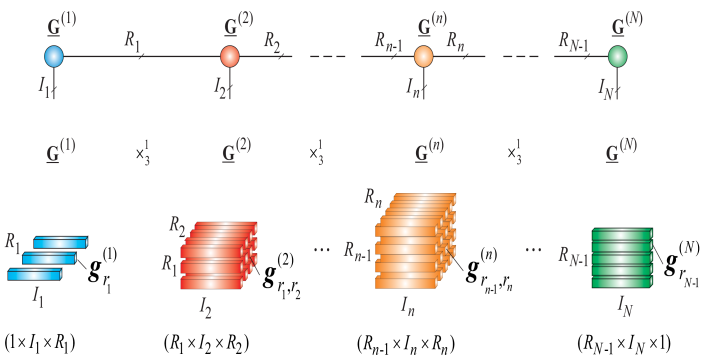
\includegraphics[width=0.45\textwidth]{img/tensor_train.png}
    \caption{Tensor Train (TT) \cite{tensorTrains, tensorTrainsOs}}
    \label{fig:tensor_trains}
\end{figure}

\section{\label{sec:problem_statement}Problem statement}

The general description of a n-qubit quantum state is given by a positive semidefinite matrix $\rho$ s.t. $Tr(\rho)=1$ with $2^{n}\times 2^{n}$ complex elements. Self-adjoint operators $M$ express observable physical quantities which can be measured experimentally. The Born rule defines a probability distribution $p_i(x_{i}=1)$ over the measurement outcomes $x_{i}$:

\begin{equation}\label{eq::Born_rule}
    p_{i} = Tr(P_{i}\rho),
\end{equation}

where $P_{i}$ are POVM measurements, $\sum_{i}P_{i}=1$. 

The expectation value of the observable $M$ is then given by the average of the eigenvalues of $M$ over the probability distribution generated by the Born rule:

\begin{equation}\label{eq::expectation_value}
    \langle M\rangle = Tr(M\rho) = \sum_{i} p_{i}m_{i},
\end{equation}

where $m_{i}$ are the eigenvalues of $M$. 

% The goal of the conventional quantum state tomography is to provide the estimate of quality of a quantum system based on the outcomes of a series of measurements.
The goal of the conventional quantum state tomography is to estimate $\rho$ given set of observations $X =\{x_i\}_{i=1}^N$.
The simple question arises: if the outcomes of the measurements are the essential source of information about a quantum system then is the complex reconstruction procedure of the density matrix really required to reproduce the observed behaviour? Scott Aaronson's work \cite{Aaronson_2007} gives the negative answer to the question and what is more important sets much easier resource requirements to the problem of approximating the measurement outcomes. The problem is reformulated in terms of PAC (probably approximately correct) learnability theory originated by Valiant \cite{Valiant1984}. We are handed $m$ samples $\{P_{k}, Tr(P_{k}\rho)\}$ called the training set $\Omega$, where $P_{k}$ are sampled from the distribution $\mathcal{D}$. This training set can be gathered experimentally by measuring the expectation values of the operators $P_{k}$. Aaronson showed that provided the training set of tuples $\{P_{k}, Tr(P_{k}\rho)\}$  we can construct a predictor $\sigma$ with probability $1-\delta$ which approximates the expectation values $Tr(P\sigma)$ with probability $\gamma$ up to precision $\epsilon$

\begin{equation}\label{eq::pac_learned_state}
    \underset{P\in\mathcal{D}}{Pr}[|Tr(P\sigma)-Tr(P\rho)|>\epsilon]\leq \gamma.
\end{equation}

The most striking result is the linear scaling of the training set size on the number of qubits $n$ in the system:

\begin{equation}\label{eq::training_set_scaling}
    m \geq \frac{const}{\epsilon^{4}\gamma^{2}}(\frac{n}{\epsilon^{4}\gamma^{2}}\log^{2}{\frac{1}{\gamma\epsilon}} + \log{\frac{1}{\delta}}).
\end{equation}

The learning of the predictor $\sigma$ if performed by minimization of an arbitrary convex function $l(\cdot)$:

\begin{equation}\label{eq::learning_loss_function}
    f = \sum_{\Omega}l(Tr(P_{k}\sigma) - Tr(P_{k}\rho)).
\end{equation}

The caveat here lies in the dimension of the matrix $\sigma$. Even though the scaling of the training set is guaranteed to scale linearly with the number of qubits the optimization has to be performed of the space of $2^{n}\times 2^{n}$ complex matrices. The storage space of the predictor grows exponentially with $n$ and the optimization quickly becomes intractable even if the problem is reduced to the semidefinite programming which has polynomial complexity solutions \cite{Nesterov1994, Groetschel1988}.

The online learning paradigm \cite{Aaronson_2019} enhances the described procedure. The updates of the predictor can be made as soon as a new sample $\{P_{k}, Tr{P_{k}\rho}\}$ arises. The estimation of the quality of a prepared quantum system can be conducted online. The outcomes from the measurements gathered during the experiment are also applicable for the learning procedure and thus we can keep tracking of the current quantum system state. 

\section{Prior work}

%The new paradigm of building the model of the unknown quantum state was introduced by Aaronson in . Many experimental tasks require knowledge of the expectation values of the particular operator sets which typically include either only single-qubit or single- and two-qubit operators. This means that the exact knowledge of the full quantum state is extremely redundant. Instead, the experimental data can be employed for building the hypothesis $\omega$ which accurately reproduces the results of the performed measurements and furthermore is capable to predict the outcome of new measurements up to the certain error level. The main result of the \cite{Aaronson_2007} states that the dataset size $m$ required for learning $\omega$ scales as $O(n)$ in the number of qubits $n$ present in the quantum system. The proposed quantum state learning approach was further developed to cover the online setting~\cite{Aaronson_2019, chen2020practical}. The online learning algorithm doesn't require to collect the whole training set for building the $\omega$ hypothesis and instead allows for updating $\omega$ after each new projector expectation value has been measured.

\begin{figure*}[ht!]
    \centering
    \includegraphics[]{img/online_learning_experiment.pdf}
    \caption{The picture a) displays the experimental setup employed for generating the dataset. The laser light of 808 nm laser diode is filtered using the single-mode fiber (SMF) and forwarded onto the preparation half of the Spatial Light Modulator (SLM). The SLM screen imposes both phase (p) and amplitude (a) holograms which convert the input gaussian mode to the predefined Hermite-Gaussian mode (see picture b)). The lenses L1, L2 and the slit pick the first diffraction order. The quarter-wave plate (QWP) and polarization beamsplitter (PBS) divert the beam towards the projection half of the SLM. The projection half applies a phase mask conjugating the input HG mode and the mode of the single-mode fiber. The signal is measure using a single-photon avalanche photodetector (SPAD). The picture b) illustrates first twelve two-dimensional modes from the Hermite-Gaussian set.}
    \label{fig:experiment}
\end{figure*}

The work \cite{Aaronson_2019} provides the complexity argument for two implementations of online learning based on the regularized follow-the-leader update algorithm (RFTL)~\cite{rftl} (Algorithm~\ref{algo:rftl} in Appendix~\ref{sec:app_algos}) and predictor matrix exponentiated gradient update alorithm (MEG)~\cite{meg} (Algorithm~\ref{algo:meg} in Appendix~\ref{sec:app_algos}). However, despite the fact that both the aforementioned algorithms are scalable w.t. number of qubits $n$, they are intractable in real experiments due to a set of specific and common reasons. The main problem of RFTL is the necessity to perform an optimization over $C_n$ in~\eqref{eq:rftl} at each step of the algorithm, which is not straightforward (here, $C_n$ is the set of all trace-1 positive semidefinite complex matrices of dimension $2^{n}\times2^{n}$). In turn, the MEG (Algorithm~\ref{algo:meg}) ensures trace-1 positive semidefinite property of the predictor $\sigma$ in \eqref{eq:meg}. However, this feature comes at the big cost. All gradient matrices are passed through the exponent which may lead to gradient explosion and numerical instability, especially in high-dimensional case.

Practical implementations of the existing online algorithms will inevitably suffer from exponentially growing $O(2^{2n})$ memory consumption due to the  need to store a full $2^n\times2^n$ predictor $\sigma$ matrix. Instead, more memory efficient low-rank approximation of $\sigma$ can be fitted.

% There exist sophisticated algorithms designed for the effective dimension reduction \cite{} which extract the symmetries hidden in the data. Another possibility lies in finding the approximate predictor $\sigma$ description which still delivers accurate approximation of the expectation values. 


The tensor networks \cite{tensorTrains, biamonte2019lectures} (Figure~\ref{fig:tensor_networks}) serve as an efficient  method to construct a low-rank approximation of the predictor. Recent works have demonstrated the benefits of using the tensor network decomposition to enhance quantum machine learning algorithms \cite{Huggins_2019} and quantum process tomography \cite{torlai2020quantum}. Artificial quantum systems typically possess the well-defined connections between the individual qubits. Knowledge of the structure of a quantum system can be employed to design the appropriate tensor network model of the system state. The particular example of the tensor network which adequately describes simple quantum systems such as linear qubit chains is the so-called matrix product state model (MPS) \cite{MPS} which is represented by {\itshape Tensor Trains (TT)}~\cite{tensorTrainsOs} (Figure~\ref{fig:tensor_trains}).

% \begin{figure}
%     \centering
%     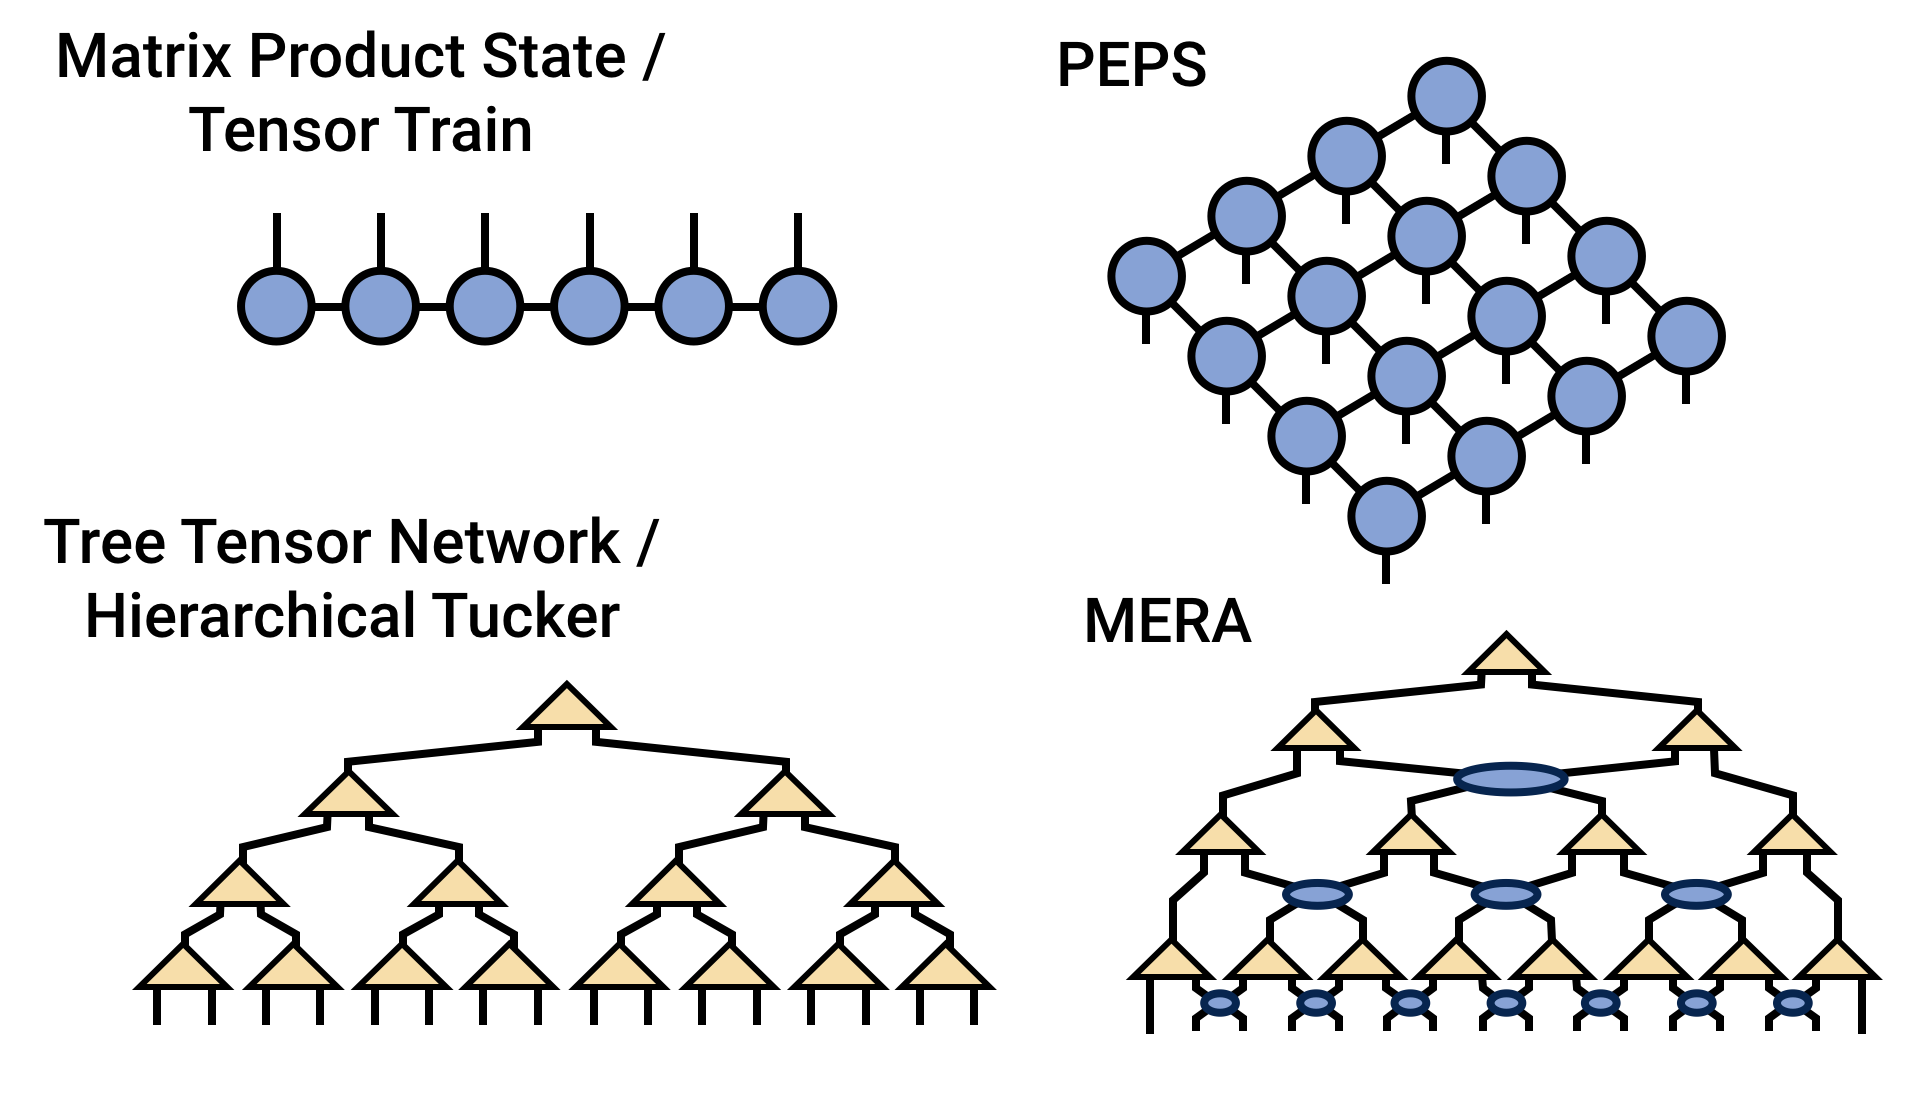
\includegraphics[width=0.45\textwidth]{img/tensor_networks.png}
%     \caption{Tensor networks types}
%     \label{fig:tensor_networks}
% \end{figure}

TT represents the sequential decomposition of the high-dimensional $d$-way tensor $\mathcal{A}\in\mathbb{R}^{n_1\times n_2\times\dots\times n_d}$ with two $2$-dimensional and $(d-2)$ $3$-dimensional tensors in the following outer product:
\begin{equation}
    \label{eq:tt}
    \mathcal{A}=\mathcal{G}^{(1)}\circ\mathcal{G}^{(2)}\circ\dots\circ\mathcal{G}^{(d)}
\end{equation}
where $\mathcal{G}^{(k)}\in\mathbb{R}^{r_{k-1}\times n_k\times r_k}$ is the $k$-th core tensor, $r_k$ are the so-called {\itshape tensor-train (TT) ranks}. The MPS with low TT ranks has shown its efficiency for simulation of the quantum circuits with moderate entanglement generation capability \cite{Waintal2020}.

In this work, we utilize TT decomposition of the quantum state. The proposed technique overcomes the exponential growth of the memory consumption and improves the optimization performance. 

\begin{figure*}[ht!]
    \centering
    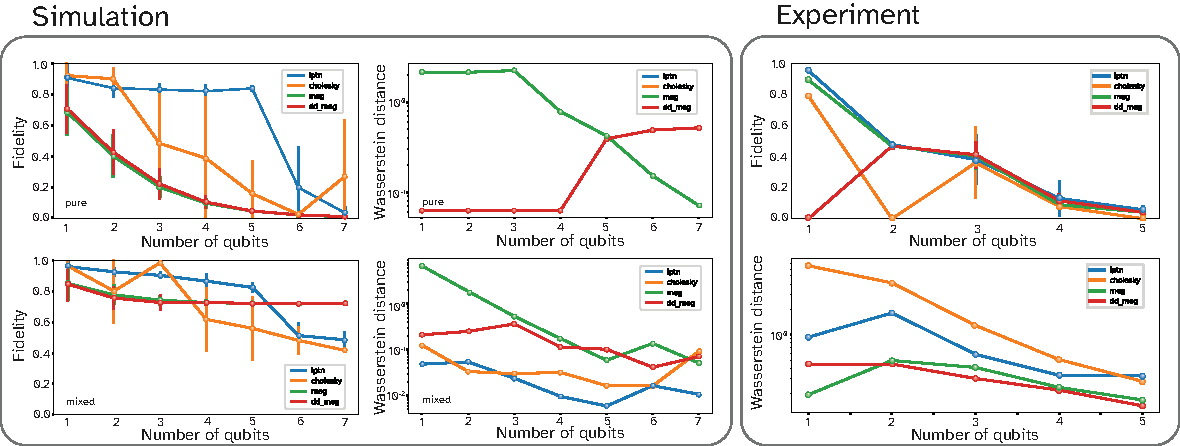
\includegraphics[width = \textwidth]{img/results.pdf}
    \caption{The panel simulation depicts the results of the numerical simulation of the comparative performance of MEG, DD-MEG, LPTN and Cholesky algorithms for pure and mixed states of up to 7 qubits. Here, the Wasserstein distance between quality distributions on train and test sets is taken. It represents an overfitting level of a model.}
    \label{fig:experiment_results}
\end{figure*} 

\section{\label{sec:algo}Learning algorithm}

In this work, we apply {\itshape locally purified tensor network} approximation to the predictor $\sigma$ in an online quantum learning experiment. Our algorithm (Algorithm \ref{algo:our}) is explicit and based on gradient descent of the low-rank approximated predictor $\sigma$.

To preserve the positivity of hypothesis $\omega$, we parametrize it in locally purified form $\sigma = X^\dagger X$, where $X$ is decomposed as a variational tensor train (TT) network. The Cholesky decomposition $\sigma = X^\dagger X$ ensures positivity of $\sigma$ for any $X$. Trace normalization of $\sigma$ can be performed analogously to MEG algorithm~\eqref{eq:meg}.

We additionally decompose $X$ into a Tensor Train according to \eqref{eq:tt}:
\begin{equation}
    X=\mathcal{G}^{(1)}\circ\mathcal{G}^{(2)}\circ\dots\circ\mathcal{G}^{(d)}
\end{equation}
where $\mathcal{G}^{(k)}\in\mathbb{R}^{r_{k-1}\times n_k\times r_k}$ is the $k$-th core tensor with $r_k$ are ranks.

% We use the Cholesky decomposition to enable positive semidefinite property of the hypothesis. The hypothesis $\omega$ is represented via the product of positive definite matrices $\omega = X^\dagger X$. The algorithm optimizes the matrix $X$ instead of direct optimization of the $\omega$. Since any $X^\dagger X$ is positive definite matrix and for any positive definite matrix Cholesky decomposition exists, we have an ensurance that fitting $X$ we will always provide positive definite hypothesis $\omega$. Trace normalization here can be performed in the same way like it was in MEG algorithm~\eqref{eq:meg}. The quantum state TT decomposition in conjunction with Cholesky decomposition is called {\itshape locally purified tensor networks} and was originally introduced in \cite{Werner_2016}.

\begin{algorithm}
\caption{Our algorithm (LPTN-QL)\\}
\label{algo:our}
\hspace*{\algorithmicindent} \textbf{Input}: $T,\eta$ \\
% \hspace*{\algorithmicindent} \textbf{Input}:\\
\begin{algorithmic}[1]
\State Set $X\coloneqq \text{TT}(2^{-n}\mathbb{I})$

\For{$t=1,\dots,T$}
    \State $\sigma \coloneqq \frac{X^\dagger X}{Tr(X^\dagger X)}$
ii    \State Consider loss function $l_t : \mathbb{R} \rightarrow \mathbb{R}$ given by measurement $E_t : l_t(Tr(E_t\sigma))$
    \State Update $X\coloneqq X-\eta\nabla_X l_t(Tr(E_t X^\dagger X))$
\EndFor

\end{algorithmic}
\end{algorithm}

The LPTN-QL algorithm was initially tested using a numerically generated set of pairs $\{P_{k}, Tr(P_{k}\rho)\}$. The unknown state $\rho$ and the two-outcomes measurements $P_{k}$ were sampled from the Haar-random distribution. The training sets for both pure and mixed states of up to 7 qubits were generated. 


% \section{\label{sec:sim}Simulations}

\section{\label{sec:exp}Experimental setup}

The performance of the Algorithm \ref{algo:our} is certified using the experimental data collected using states of light encoded in the transverse Hermite-Gaussian ($HG$) spatial modes. The $HG_{mn}(x,y)$ modes constitute discrete orthonormal basis in transverse spatial coordinates, where indices $m,n$ enumerate modes in $X$ and $Y$ axes respectively. Each mode is identified by the order $k = m+n$. The maximal order mode we prepare in the experiment depends on the dimensionality $D$ of the quantum system under study. Given the required dimension value $D$ the $k_{max}$ is the minimal integer number satisfying the inequality $(k_{max}+1)(k_{max}+2)/2 \geq D$. We have tested the algorithm \ref{algo:our} using the state dimensions $D =2,4,8,16,32$, which correspond to $n=1,2,3,4,5$ qubits in the system.

The experimental setup is illustrated in Fig. \ref{fig:experiment}. We use weak coherent states of light produced by the 808 nm laser diode. The spatial mode of the diode beam is filtered using the single-mode fiber (SMF-1). We employ the single spatial light modulator (SLM) to enable both state preparation and measurement in $HG_{mn}$ mode basis. The top half of the SLM reflective liquid crystal screen displays the hologram designed for preparation of the desired state and the bottom half in pair with the single-mode fiber (SMF-2) implements the projective measurements \cite{Bent2015, Palmieri2020}. The holograms on the SLM include blazed grating to induce beam mode amplitude modulation \cite{Bolduc2013} thus we use the pinhole to select only the first diffraction order. We note that optimal $HG$ mode preparation and measurement is achieved only after the Gouy phase of the beam is taken into account \cite{Struchalin2020}.

\section{Results}

The experiments are performed on three types of datasets. The first type consists of simulated data of the pure state learning case. The second one includes simulated data for the mixed state case. The simulated datasets are generated by projecting the quantum state $\rho$ onto Haar-random sampled vectors $\left|\chi_{i}\right\rangle$. The size of the simulated systems varies from $1$ to $7$ qubits. The projectors number spans the interval $[1, n\_qubits\times1000]$ ($10$ values picked uniformly in log scale). The third dataset is comprised of experimental measurements on systems with number of qubits ranging from $1$ to $5$. The measurements were conducted using the setup described in \ref{sec:exp}.

We have tested four algorithms: the well-known Matrix Exponentiated Gradient (MEG,~\cite{meg}) and Doubling trick MEG (DD-MEG,~\cite{ddmeg}) and two distinct implementations of our algorithm. The first implementation (LPTN-QL) uses Tensor Train decomposition of $X$ in hypothesis $\sigma = X^\dagger X$. Tensor rank of $X$ decomposition varies from $1$ to $2^{n\_qubits+2}$ in each experiment ($10$ values picked uniformly in log scale). The second implementation (Cholesky) fits complete $X$ of $\sigma = X^\dagger X$ without any decomposition.

Each dataset is splitted into two parts - training and validation sets. The first part is served as a training set for learning the predictor $\sigma$. The elements of the second set were used to run the validation procedure which proves the predictive strength of the $\sigma$. The Fig. \ref{fig:experiment_results} summarizes the results of the experiment. 

In this work, several criteriums were experimentally verified: quality, overfitting, minimal and sufficient training size, scalability w.t. qubits number, training speed, RAM and GPU memory consuption and training time. 

\begin{figure}
    \centering
    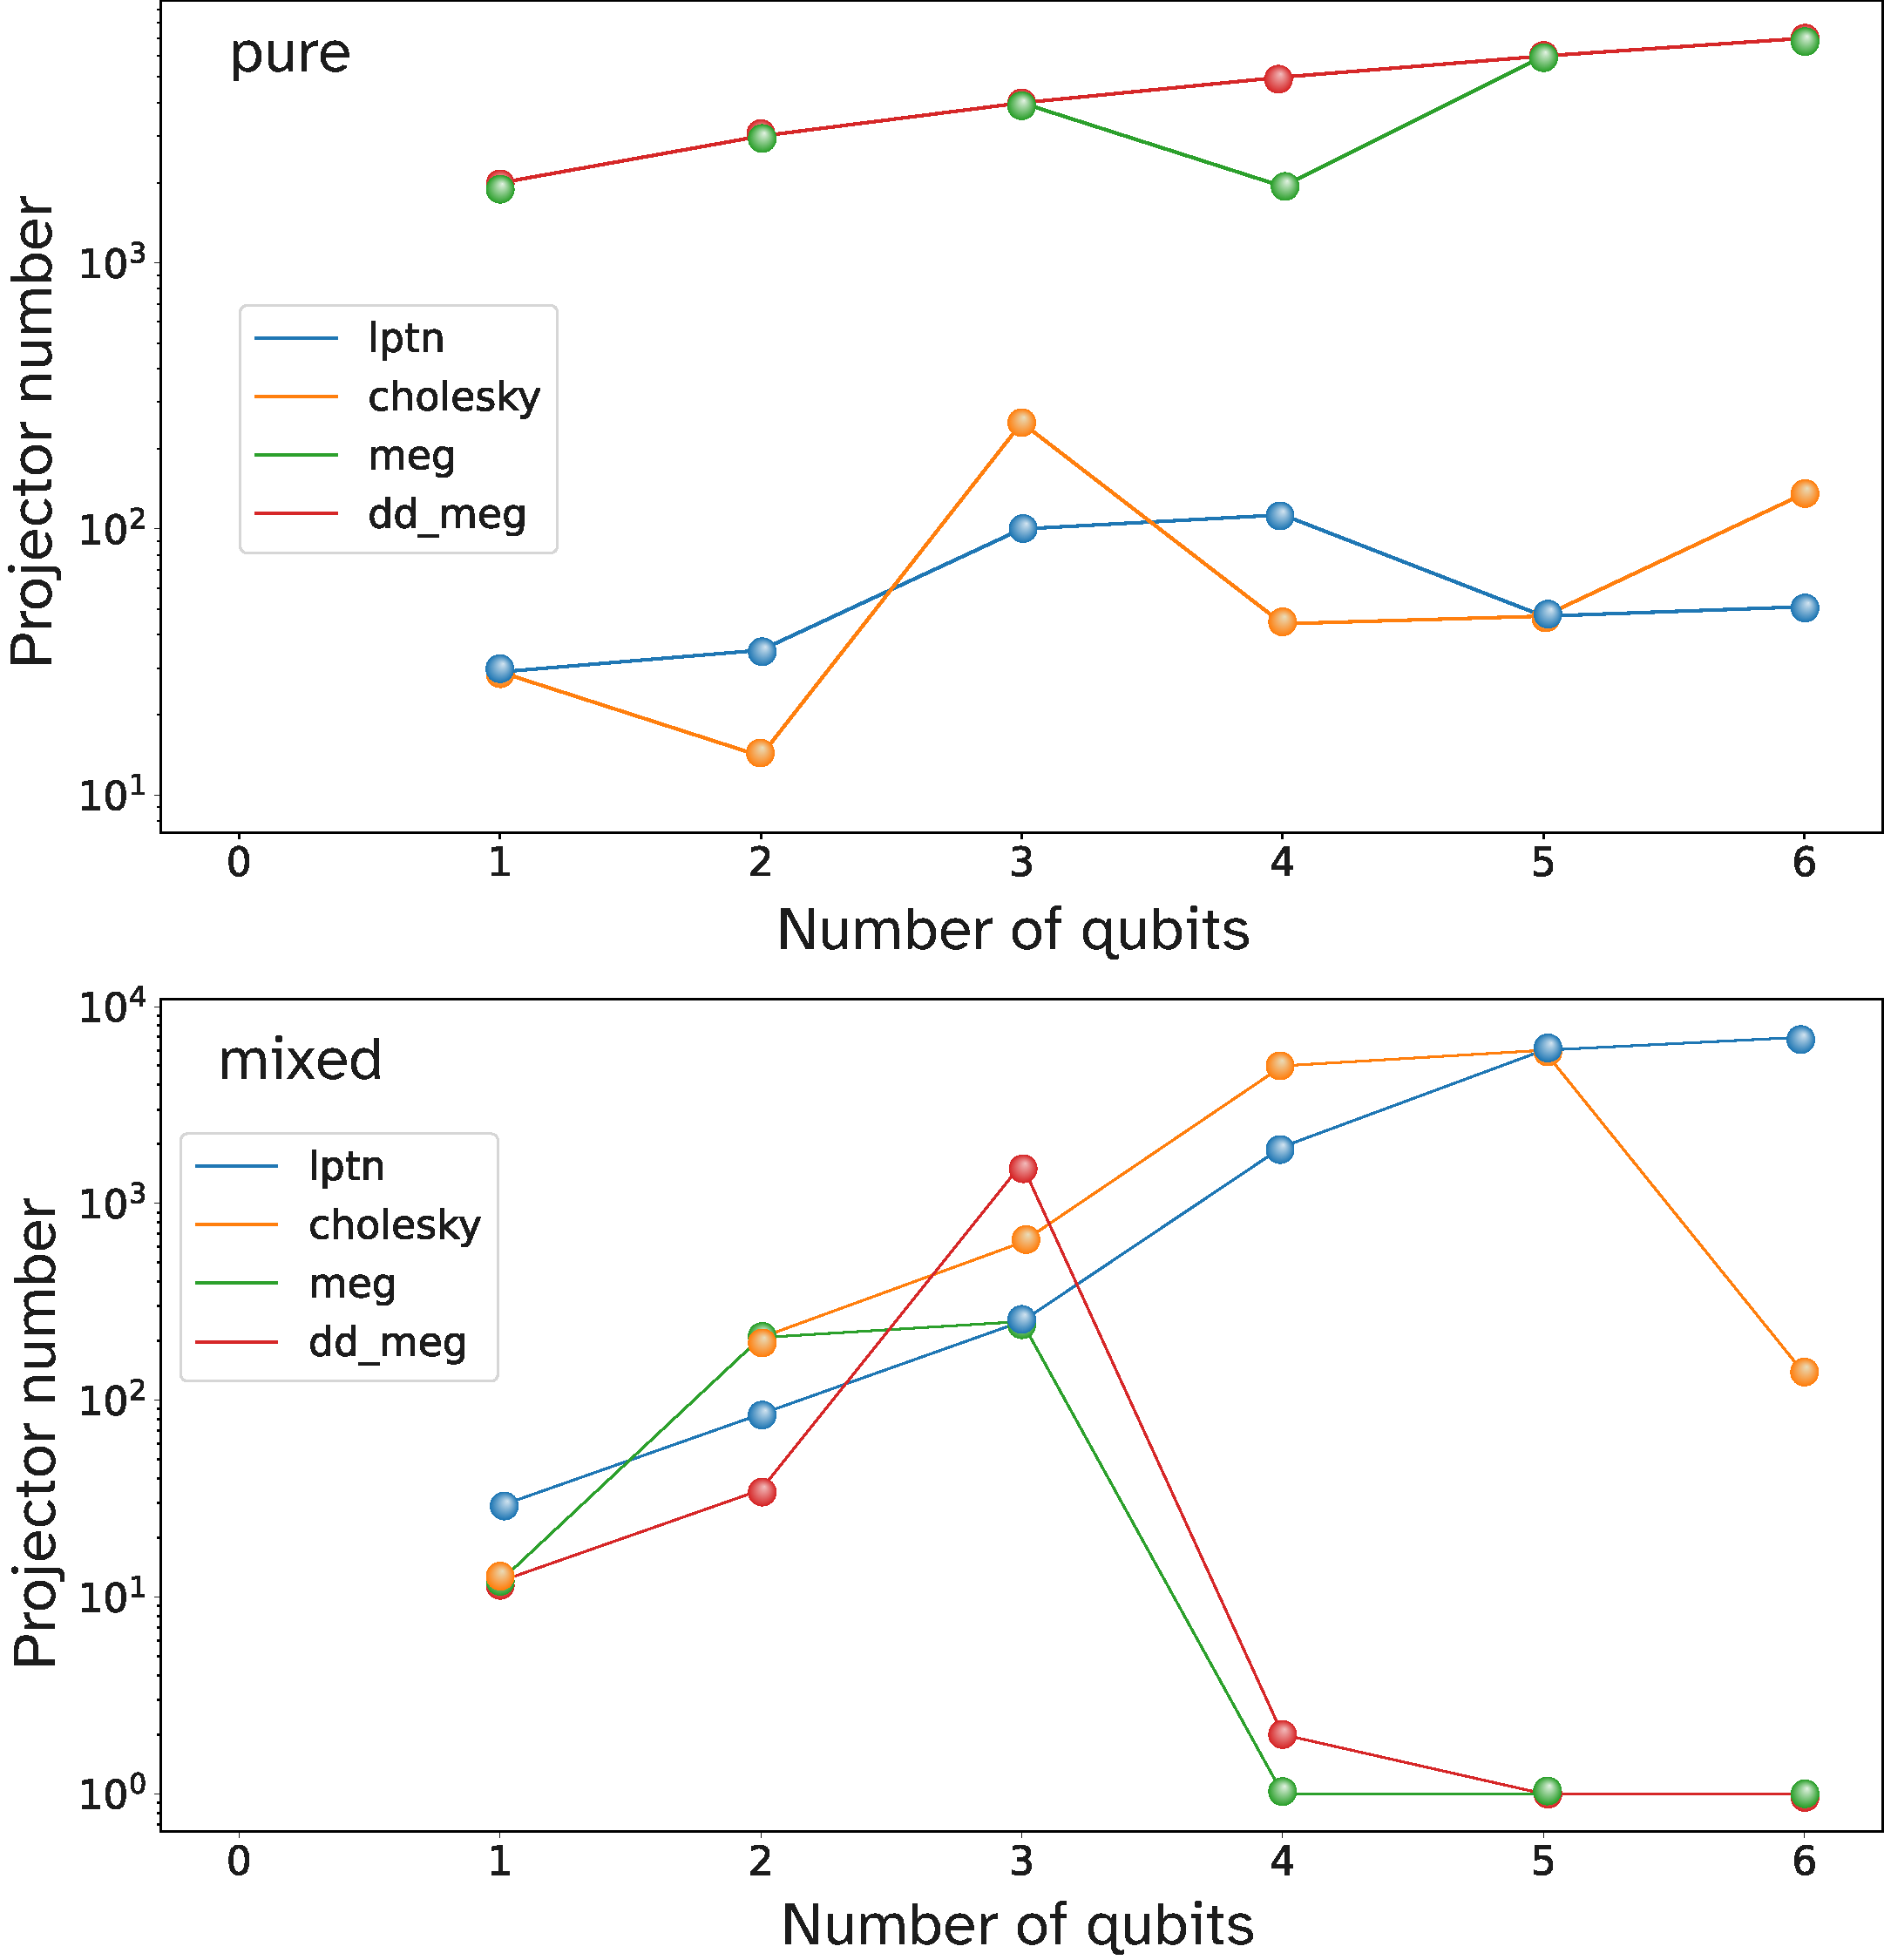
\includegraphics[width=0.45\textwidth]{img/sufficient_projectors_cnt_clean.pdf}
    \caption{The plots of the sufficient projector number versus the number of qubits in the system.}
    \label{fig:sufficient_projectors}
\end{figure}

We use the fidelity measure $\mathcal{F}(\sigma,\rho)=(Tr\sqrt{\sqrt{\rho}\sigma\sqrt{\rho}})^2$ to estimate the closeness of the predictor to the reference state. The reference state was either generated numerically during the simulations or was reconstructed from the measurement data \cite{Kovlakov2018}.

% Overfitting
In order to estimate overfitting, the projections distributions on train and test set of projectors are compared. Since projection measurements are Bernoulli distributed according to Born rule, t-test for two Bernoulli distributions are used for each projector $x_i$:
\begin{equation}
    U_{x_i} = \frac{\frac{M_{x_i}^{\rho}}{N_{x_i}^{\rho}}-\frac{M_{x_i}^{\sigma}}{N_{x_i}^{\sigma}}}{\sqrt{p(1-p)(\frac{1}{N_{x_i}^{\rho}}+\frac{1}{N_{x_i}^{\sigma}})}}
\end{equation}
where $M_{x_i}^{\rho}$ is a number of successful outcomes for projection of real state $\rho$, $N_{x_i}^{\rho}$ is a total number of measurements of $\rho$ for a given projector $x_i$, $M_{x_i}^{\sigma}$ is a number of successful outcomes for projection of fitted hypothesis $\sigma$, $N_{x_i}^{\sigma}$ is a total number of measurements of $\sigma$ for a given projector $x_i$, $p=\frac{M_{x_i}^{\rho}}{N_{x_i}^{\rho}}$.
After, the Wasserstein distance between $\{U_{x_i}|x_i\in X^{train}\}$ and $\{U_{x_i}|x_i\in X^{test}\}$ distributions is measured (Figure \ref{fig:experiment_results}b).

% Minimal and sufficient training size

We used the dependence of the fidelity value $\mathcal{F}(\sigma,\rho)$ on the projector number to estimate a sufficient amount of measurements which need to be performed for building a good predictor. The plots for pure and mixed states illustrated in Fig.\ref{fig:sufficient_projectors} indicate subexponential growth of the sufficient training set size.

% Scalability w.t. qubits number, training speed, RAM and GPU memory consuption and training time

The technical details covering RAM and GPU memory consumption and training time can be found in appendix \ref{sec:app_memory}.

\section{\label{sec:discuss}Discussion}

We have designed and implemented experimentally the online learning algorithm based on locally purified tensor networks. We have tested the performance of the developed algorithm using simulated and experimentally measured datasets.

The LPTN-QL algorithm shows superior prefromance opposed to the previously reported MEG and DD-MEG algorithms in terms the required training set size (see Fig.\ref{fig:sufficient_projectors}). 


\section{\label{sec:acknowledge}Acknowledgements}

\bibliography{apssamp}% Produces the bibliography via BibTeX.

\appendix

\section{The reported algorithms}
\label{sec:app_algos}

\begin{algorithm}
\caption{Regularized Follow-the-Leader\\ RFTL,~\cite{rftl}}
\hspace*{\algorithmicindent} \textbf{Input}: $T,\mathcal{K}\coloneqq C_n,\eta < \frac{1}{2}$ \\
% \hspace*{\algorithmicindent} \textbf{Input}:\\
\begin{algorithmic}[1]
\State Set $\omega_1\coloneqq 2^{-n}\mathbb{I}$

\For{$t=1,\dots,T$}
    \State  Predict $\omega_t$. Consider the convex and L-Lipschitz loss function $l_t : \mathbb{R} \rightarrow \mathbb{R}$ given by measurement $E_t : l_t(Tr(E_t\phi))$. Let $l_t'(x)$ be a sub-derivative of $l_t$ with respect to $x$. Define
    $$\nabla_t\coloneqq l'_t(Tr(E_t\omega_t))E_t$$

\State Update decision according to the RFTL rule with von Neumann entropy:
\begin{equation}
\label{eq:rftl}
  \omega_{t+1}\coloneqq\argmin_{\phi\in\mathcal{K}}{\big\{ \eta\Sigma_{s=1}^tTr(\nabla_s\phi)+\Sigma_{i=1}^{2^n}\lambda_i(\phi)log\lambda_i(\phi) \big\}}  
\end{equation}

\EndFor

\end{algorithmic}
\label{algo:rftl}
\end{algorithm}

\begin{algorithm}
\caption{Matrix Exponentiated Gradient updates\\ MEG,~\cite{meg}}
\hspace*{\algorithmicindent} \textbf{Input}: $T,\mathcal{K}\coloneqq C_n,\eta < \frac{1}{2}$ \\
% \hspace*{\algorithmicindent} \textbf{Input}:\\
\begin{algorithmic}[1]
\State Set $\omega_1\coloneqq 2^{-n}\mathbb{I}$

\For{$t=1,\dots,T$}
    \State  Predict $\omega_t$. Consider the convex and L-Lipschitz loss function $l_t : \mathbb{R} \rightarrow \mathbb{R}$ given by measurement $E_t : l_t(Tr(E_t\phi))$. Let $l_t'(x)$ be a sub-derivative of $l_t$ with respect to $x$. Define
    $$\nabla_t\coloneqq l'_t(Tr(E_t\omega_t))E_t$$

\State Update decision according to the RFTL rule with von Neumann entropy:
\begin{equation}
\label{eq:meg}
\omega_{t+1}\coloneqq\frac{exp(-\frac{\eta}{L}\Sigma_{s=1}^t\nabla_s)}{Tr(exp(-\frac{\eta}{L}\Sigma_{s=1}^t\nabla_s))}    
\end{equation}

\EndFor

\end{algorithmic}
\label{algo:meg}
\end{algorithm}

\section{Memory consumption}\label{sec:app_memory}

\end{document}
%
% ****** End of file apssamp.tex ******

